% $Header: /home/vedranm/bitbucket/beamer/solutions/generic-talks/generic-ornate-15min-45min.en.tex,v 90e850259b8b 2007/01/28 20:48:30 tantau $

\documentclass{beamer}

% This file is a solution template for:

% - Giving a talk on some subject.
% - The talk is between 15min and 45min long.
% - Style is ornate.



% Copyright 2004 by Till Tantau <tantau@users.sourceforge.net>.
%
% In principle, this file can be redistributed and/or modified under
% the terms of the GNU Public License, version 2.
%
% However, this file is supposed to be a template to be modified
% for your own needs. For this reason, if you use this file as a
% template and not specifically distribute it as part of a another
% package/program, I grant the extra permission to freely copy and
% modify this file as you see fit and even to delete this copyright
% notice.


\mode<presentation>
{
  \usetheme{Warsaw}
  % or ...

  \setbeamercovered{transparent}
  % or whatever (possibly just delete it)
}

      \theoremstyle{theorem}
      \newtheorem{proposition}[theorem]{Proposition}
      \theoremstyle{definition}
      \newtheorem{game}[theorem]{Game}
      \newtheorem{question}[theorem]{Question}

\usepackage[english]{babel}
% or whatever

\usepackage[latin1]{inputenc}
% or whatever

\usepackage{times}
\usepackage[T1]{fontenc}
% Or whatever. Note that the encoding and the font should match. If T1
% does not look nice, try deleting the line with the fontenc.


\usepackage{marvosym} % For \Smiley
\usepackage{verbatim} % for \verbatiminput

\title
{IBL \& Active Learning with Math Puzzles}

\subtitle
{at Lamar University} % (optional)

\author%[Author, Another] % (optional, use only with lots of authors)
{Steven~Clontz~\\http://stevenclontz.com}%\inst{1} \and S.~Another\inst{2}}
% - Use the \inst{?} command only if the authors have different
%   affiliation.

\institute[Auburn University] % (optional, but mostly needed)
{
  %\inst{1}%
  Department of Mathematics and Statistics\\
  Auburn University}
  %\and
  %\inst{2}%
  %Department of Theoretical Philosophy\\
  %University of Elsewhere}
% - Use the \inst command only if there are several affiliations.
% - Keep it simple, no one is interested in your street address.

\date[15-04-24] % (optional)
{April 24, 2015}


% If you have a file called "university-logo-filename.xxx", where xxx
% is a graphic format that can be processed by latex or pdflatex,
% resp., then you can add a logo as follows:

 % \pgfdeclareimage[height=1cm]{university-logo}{auburn_logo.png}
 % \logo{\pgfuseimage{university-logo}}



% Delete this, if you do not want the table of contents to pop up at
% the beginning of each subsection:
%\AtBeginSubsection[]
%{
%  \begin{frame}<beamer>{Outline}
%    \tableofcontents[currentsection,currentsubsection]
%  \end{frame}
%}


% If you wish to uncover everything in a step-wise fashion, uncomment
% the following command:

%\beamerdefaultoverlayspecification{<+->}

% My game notational definitions
\newcommand{\win}{\uparrow}
\newcommand{\prewin}{\uparrow_{\text{pre}}}
\newcommand{\markwin}{\uparrow_{\text{mark}}}
\newcommand{\tactwin}{\uparrow_{\text{tact}}}
\newcommand{\ktactwin}[1]{\uparrow_{#1\text{-tact}}}
\newcommand{\kmarkwin}[1]{\uparrow_{#1\text{-mark}}}
\newcommand{\codewin}{\uparrow_{\text{code}}}
\newcommand{\limitwin}{\uparrow_{\text{limit}}}
\newcommand{\oneptcomp}[1]{#1^*}
\newcommand{\oneptlind}[1]{#1^\dagger}
\newcommand{\congame}[2]{Con_{\pl O\pl P}(#1,#2)}
\newcommand{\clusgame}[2]{Clus_{\pl O\pl P}(#1,#2)}
\newcommand{\lfkpgame}[1]{LF_{\pl K\pl P}(#1)}
\newcommand{\lfklgame}[1]{LF_{\pl K\pl L}(#1)}
\newcommand{\pfgame}[1]{PF_{\pl F\pl C}(#1)}
\newcommand{\mengame}[1]{Cov_{\pl C\pl F}(#1)}
\newcommand{\rothgame}[1]{Cov_{\pl C\pl S}(#1)}
\newcommand{\altrothgame}[1]{Cov_{\pl P\pl O}(#1)}
\newcommand{\fillgame}[1]{Fill^{\subseteq}_{\pl M\pl N}(#1)}
\newcommand{\sfillgame}[1]{Fill^{\subsetneq}_{\pl M\pl N}(#1)}
\newcommand{\kfillgame}[1]{Fill^{\subseteq}_{\pl C\pl F}(#1)}
\newcommand{\ksfillgame}[1]{Fill^{\subsetneq}_{\pl C\pl F}(#1)}
\newcommand{\recallgame}[2]{Rec^{#1}_{\pl F\pl S}(#2)}
\newcommand{\sigmaprodr}[1]{\Sigma\mathbb{R}^{#1}}
\newcommand{\sigmaprodtwo}[1]{\Sigma2^{#1}}
\newcommand{\concat}{^\frown}
\newcommand{\rest}{\restriction}
\newcommand{\cl}[1]{\overline{#1}}
\newcommand{\pow}[1]{\mc{P}(#1)}
\newcommand{\<}{\langle}
\renewcommand{\>}{\rangle}
\newcommand{\al}[1]{{#1}^*}
\newcommand{\mc}[1]{\mathcal{#1}}
\newcommand{\po}{\mathbb{P}}
\newcommand{\pok}{\po_\kappa}
\newcommand{\Lim}{\mathrm{Lim}}
\newcommand{\Suc}{\mathrm{Suc}}
\newcommand{\ds}{\displaystyle}
\newcommand{\alcomp}{\al\parallel}
\newcommand{\rank}{\textrm{rank}}
\newcommand{\dom}{\textrm{dom}}
\newcommand{\scish}{almost-$\sigma$-(relatively compact)}

\usepackage{mathrsfs}
\newcommand{\pl}[1]{\mathscr{#1}}

\newcommand{\vpause}{\pause\vspace{1em}}

\newcommand{\term}[1]{\textbf{#1}}




\begin{document}
% \renewcommand{\pause}{}

\begin{frame}
  \titlepage
\end{frame}

% \begin{frame}{Table of Contents}
%   \tableofcontents
%   % You might wish to add the option [pausesections]
% \end{frame}

\section{Puzzle: Safe and Secured}

\begin{frame}{Safe and Secured}
  You're on the tail of the vicious supercriminal Insert Name Here!

  \vpause

  At the entrance to his/her secret lair, you find a strange combination
  lock. Fortunately, Insert Name Here is pretty forgetful, so you also find
  a post-it note with this hint for the combination:

  \vpause

  \textit{%
    correct combination uses exactly one of each symbol / letter /
    character per row and column.
  }

  \vpause

  Can you crack the code and access Insert Name Here's hideaway?
\end{frame}

\begin{frame}
  \centerline{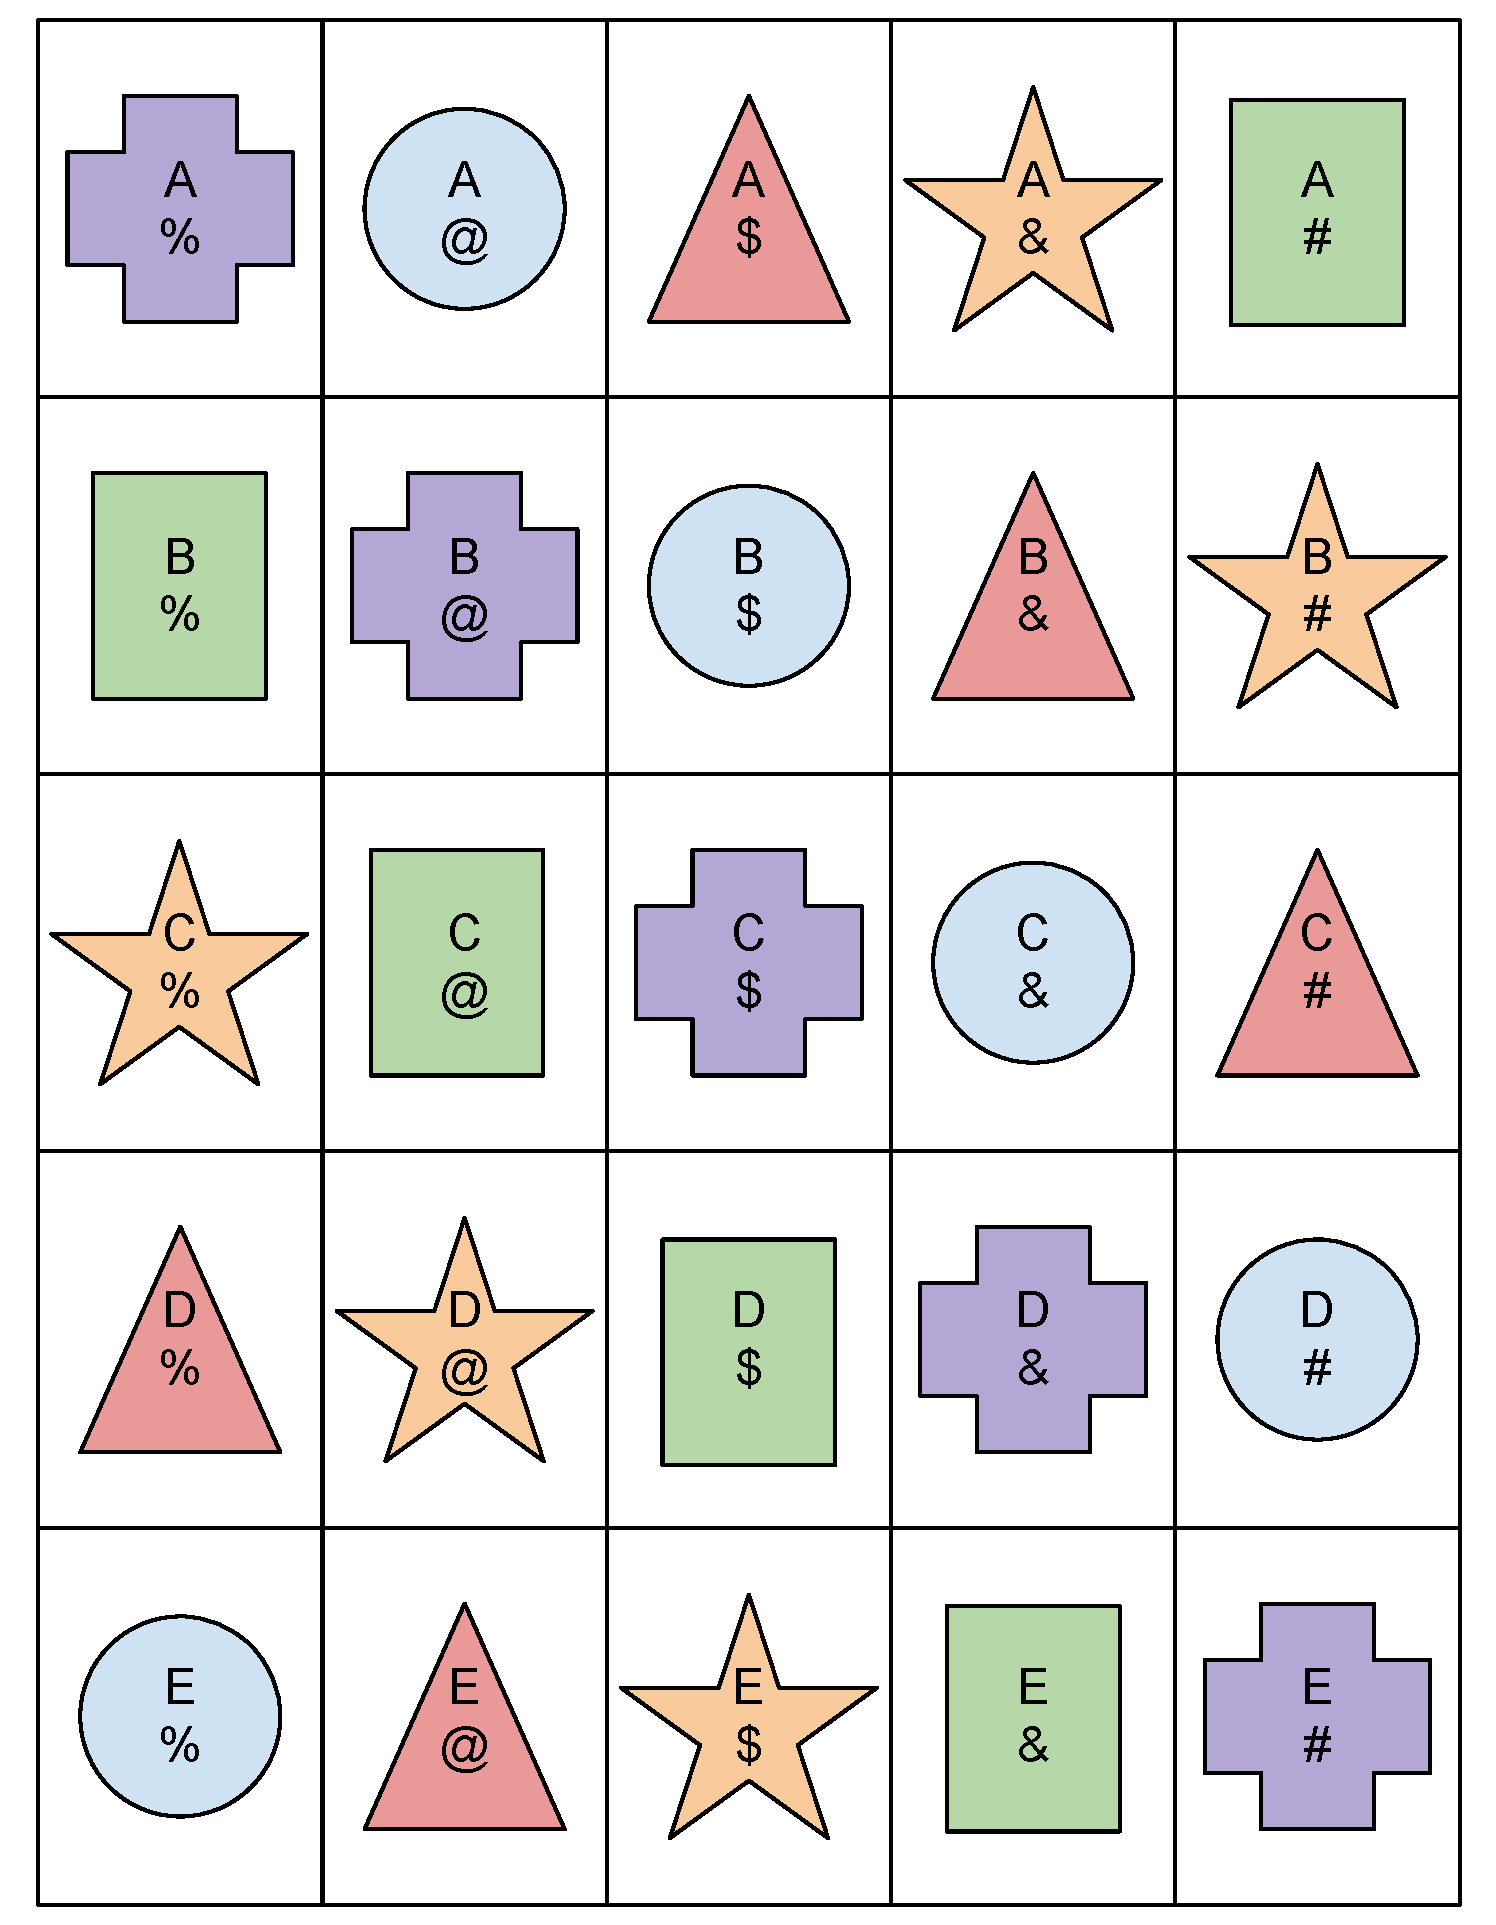
\includegraphics[height=3in]{safeAndSecured.pdf}}
\end{frame}

\section{Puzzlehunts}

\subsection{About puzzlehunts}

\begin{frame}
  A \textbf{puzzlehunt}, also known as a puzzle race,
  puzzle party, or mystery hunt, is a type of scavenger hunt where instead
  of a list of items to collect, players
  are presented with a number of puzzles to solve.

  \vpause

  Since this is a hunt, usually the puzzles are hidden in a physical
  location within certain boundaries (campus, city, building), or the
  solutions send players to hidden locations to find some sort of token,
  or both!
\end{frame}

\begin{frame}
  Famous puzzlehunts include the MIT Mystery Hunt and the
  Microsoft College Puzzle Challenge.

  \vpause

  Some puzzlehunts are organized by communities of puzzle solvers,
  and others are sponsored by companies.

  \vpause

  Increasingly, businesses are using puzzles as a way to determine if
  future employees are able to problem-solve (as opposed to assessing
  prior knowledge).
\end{frame}

\subsection{Mathematics and Puzzles}

\begin{frame}
  Designing math problems and puzzles are very similar processes.

  \pause

  \begin{itemize}
    \item What do we want to design our problem/puzzle about?
      \begin{itemize}
        \item Integration
        \item Morse code
      \end{itemize}
    \pause
    \item How should I present the problem so it isn't trivial?
      \begin{itemize}
        \item Ask about area under a curve
        \item Embed it as punctuation within a paragrapht
      \end{itemize}
    \pause
    \item How do I make sure the player/student doesn't get off-track?
      \begin{itemize}
        \item Ask to prove that it equals \(10\)
        \item Hint system
      \end{itemize}
  \end{itemize}
\end{frame}

\begin{frame}
  Many players report added satisfaction with a puzzle if they feel like they
  learned something new along the way (without it feeling like an exam).

  \vpause

  Likewise, a math problem should be designed like a (good) puzzle: students
  should feel that it was designed to be solved, not to confound.
\end{frame}

\section{Mathematical Puzzlehunts}

\subsection{AMP'd and LaMP}

\begin{frame}
  The AMP'd (Auburn Mathematical Puzzle) Challenge was founded in 2012
  when attempting to adapt a weekend-long IBL math camp format into
  a day-long math competition. High school and middle school events
  are held each year, and the LaMP (Lamar Mathematical Puzzle) Challenge
  high school event will run in April 2015.

  \vpause

  Rather than asking individual students to sit at a desk for two hours
  and work abstract mathematical problems, teams of students collaborate
  on puzzles by (incidentally) modeling them with mathematics.
\end{frame}

\subsection{LaMP Format}

\begin{frame}{LaMP Format}

  \begin{itemize}
    \item
    Opening Puzzle

    A physical challenge requiring students to run around a green space
    to collect the data required to solve an otherwise quick puzzle.
    Teams must quickly submit a solution to earn points and
    unlock the main game.

    \pause

    \item
    Main Puzzles

    Teams receive a packet of mathematical puzzles. Each solution unveils
    a secret message worth points, and solving the riddle within reveals
    the hidden location of an EXTRA Puzzle somewhere on campus.

  \end{itemize}
\end{frame}

\begin{frame}{LaMP Format (cont.)}

  \begin{itemize}
    \item
    EXTRA Puzzles

    Extensions to the main puzzles, typically optimization puzzles.
    Teams which submit the best solution earn points.

    \pause

    \item
    Metapuzzle

    An undergraduate-level mathematics problem from a field
    unrepresented at the high school level. Hints are provided to teams
    as main Puzzles are solved, and points are awarded based on the
    generality of the submited solutions.
  \end{itemize}
\end{frame}

\subsection{Moving forward}

\begin{frame}
  The LaMP event will expand in 2016 to involve multiple campuses
  across the country.

  \vpause

  We're planning a web application to manage the game, as well
  as allow teams to optionally play
  from their schools if there isn't an event nearby.

  \vpause

  Eventually, we'd like to involve elaborate manipulative puzzles
  and support regional/national competitions for top teams.
\end{frame}

\section{Puzzle Solution}

\begin{frame}\small
  \centerline{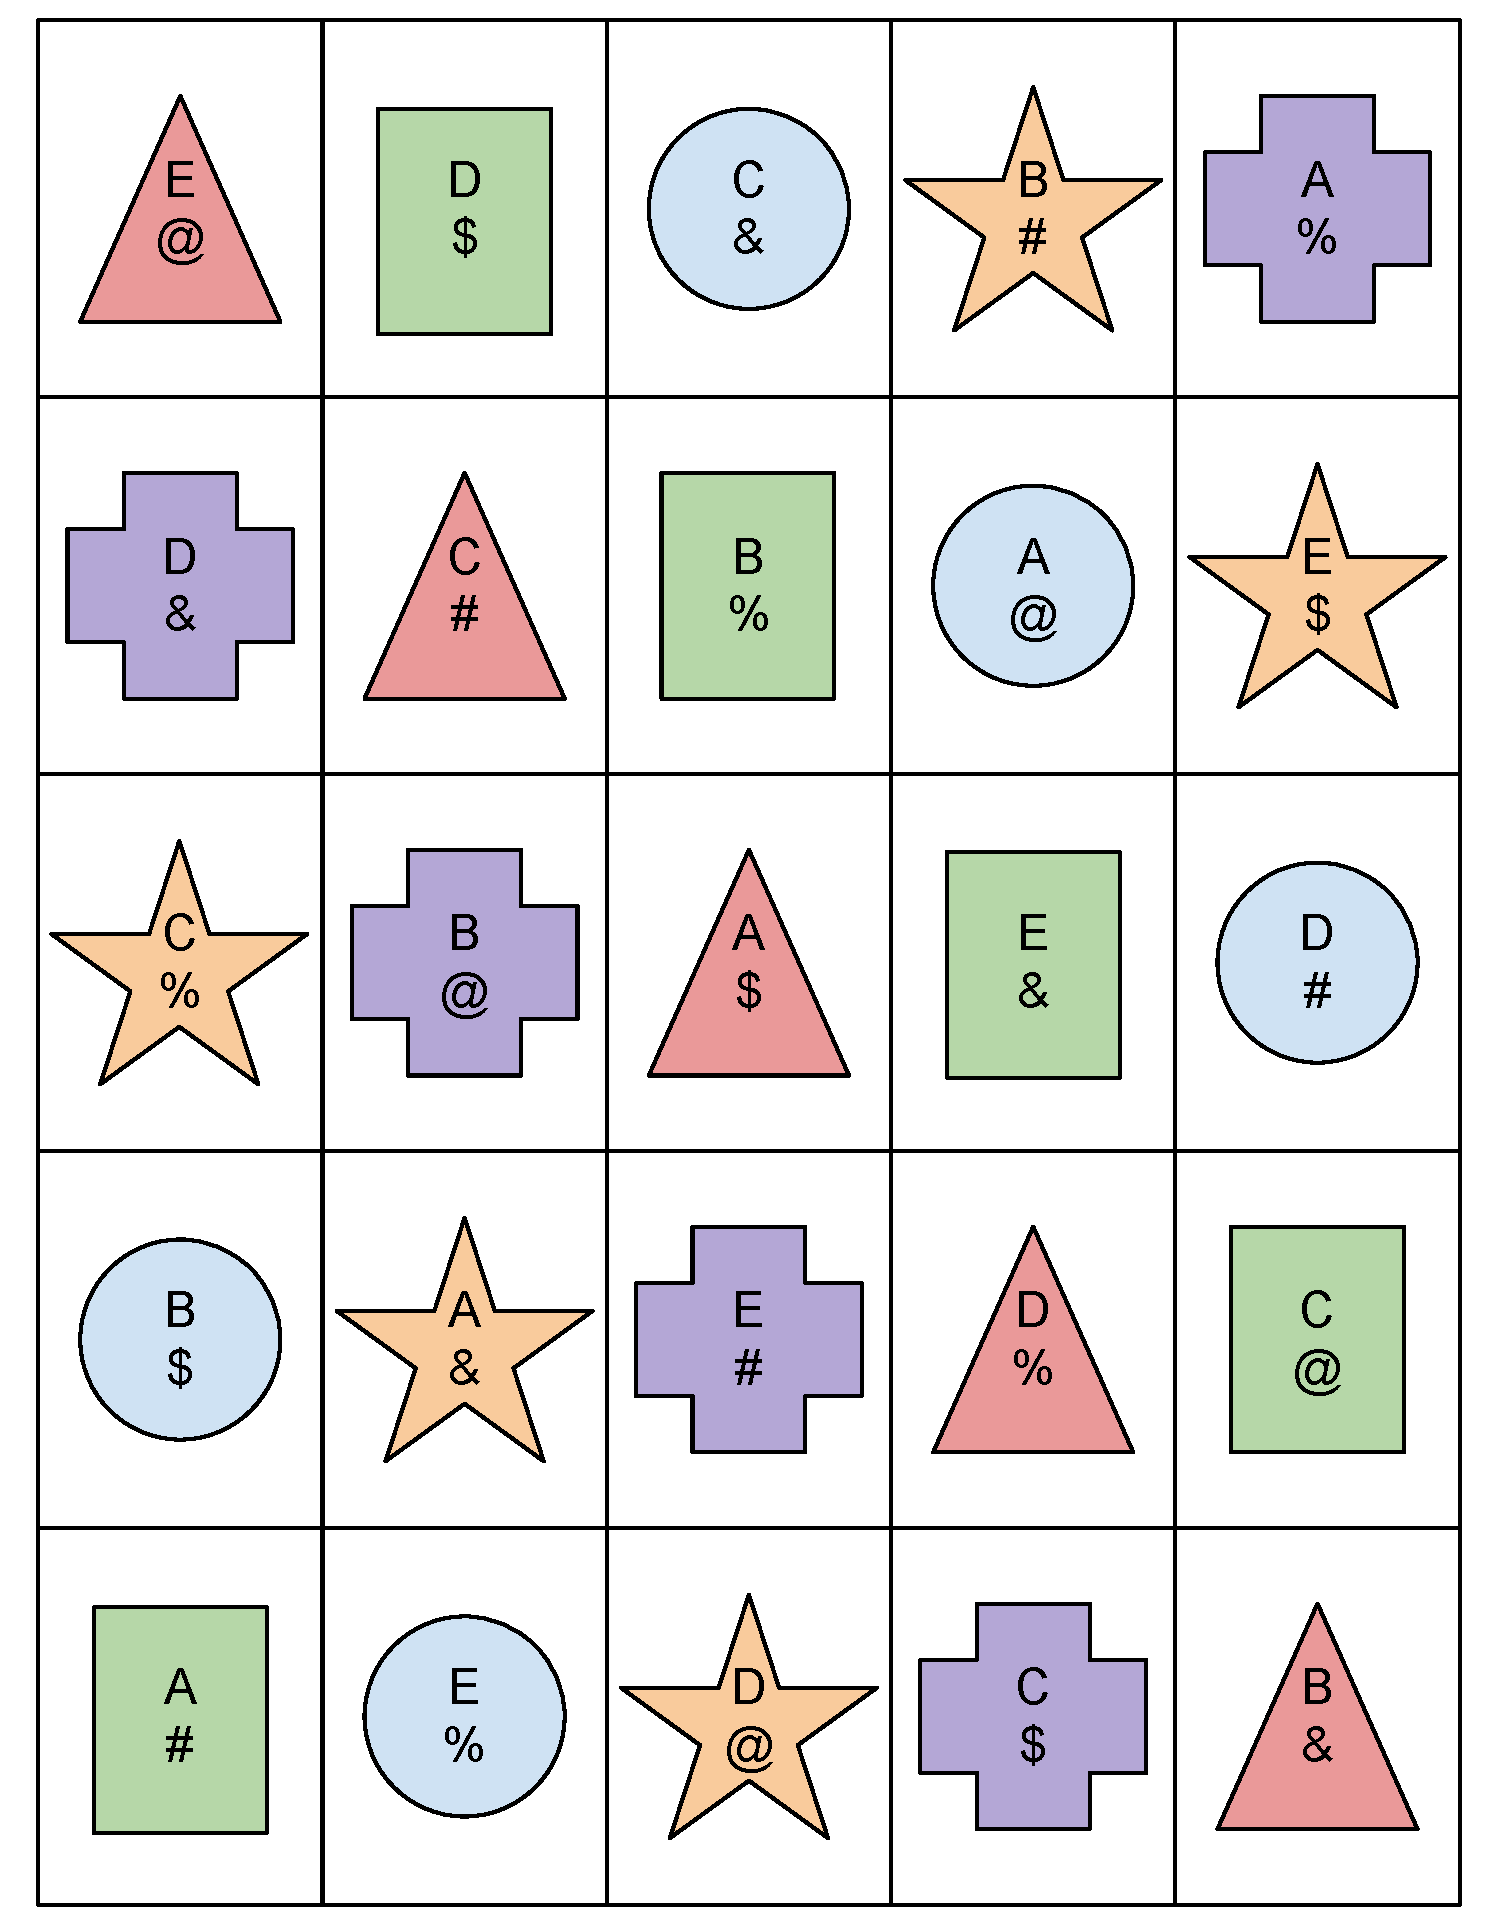
\includegraphics[height=2in]{safeAndSecuredSol.pdf}}

  \pause

  EXTRA Puzzle: Add numbers 1-5 which appear with each column, row,
  shape, letter, and symbol exactly once!

  \vpause

  By the way, this is an example of using \textit{mutually orthogonal
  Latin squares}, a topic from Design Theory.
\end{frame}

\section*{}

\begin{frame}
Questions? Thanks for having me!
\end{frame}


\end{document}


